% !TEX root =  master.tex
\chapter{Einleitung}
Diese Arbeit besch"aftigt sich mit dem "Uberpr"ufen der L"osbarkeit einer Instanz des 15-Puzzles. Zun"achst wird der historische Hintergrund beleuchtet, anschlie"send wird der Algorithmus von Herrn Bradlow vorgestellt und das notwendige Vorgehen anhand von Beispielen dargestellt.\\
Abschlie"send wird die Implementierung und das Testen der Umsetzung des Algorithmus' in der Programmiersprache Python beschrieben.
\section{Geschichte} % (fold)
\label{cha:Geschichte}
Die erste bekannte Erscheinung des heute so bekannten Puzzels ist in den 1870'er Jahren in Amerika aufgetreten. Bisher ist man davon ausgegangen, dass der Erfinder des Puzzels der Amerikaner Sam Loyd ist, jedoch ist nach einer Untersuchung von Jerry Slocum and Dieter Gebhardt Sam Loyd gar nicht der echte Erfinder des 15-Puzzels \autocite{anchor-puzzle:book, the-15-puzzle:online}. Demnach hat Sam Loyd die Idee nur gut vermarktet und sich selbst dadurch in die "Offentlichkeit gestellt \autocite{wiki-15-puzzle:online}.\\
\texttt{zitat? -> woher die information}
Nichtsdestotrotz hat Sam Loyd es geschafft die Aufmerksamkeit der "Offentlichkeit auf das Puzzel zu lenken und somit das Interesse vieler geweckt.\\
Das Ziel des Puzzels ist es 15 Puzzelsteine numeriert von 1-15 auf einer 4 x 4 Ebene durch Verschiebung in seine Urspr"ungliche sortierte Form zur"uckzubringen (vgl. Abb.\ref{fig:puzzle-end}).
\begin{figure}[H]
    \centering
    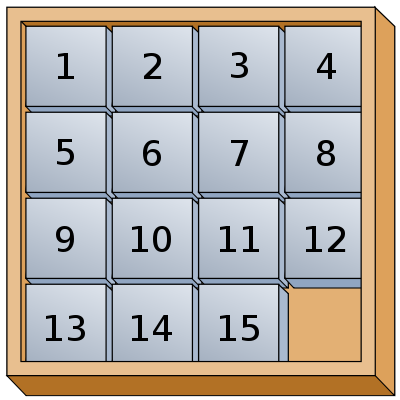
\includegraphics[width=.3\textwidth,keepaspectratio]{img/Fifteen_puzzle.png}
    \captionsetup{format=hang}
    \caption[Zielzustand des 15 Puzzels]{\label{fig:puzzle-end}Zielzustand des 15 Puzzels}
\end{figure}
Der schnelle Ruhm des Puzzels ergab sich nun daraus, dass Sam Loyd ein Preisgeld von \$$1000$ f"ur denjenigen ausschrieb, der sein Puzzel l"osen kann. Darauf folgte ein "offentlicher Ansturm auf das Puzzel, welches als \enquote{14-15 Puzzel} bekannt wurde, da lediglich die 14 und 15 vertauscht wurden. (Vgl. Abb.\ref{fig:puzzle-illustration})
\begin{figure}[H]
    \centering
    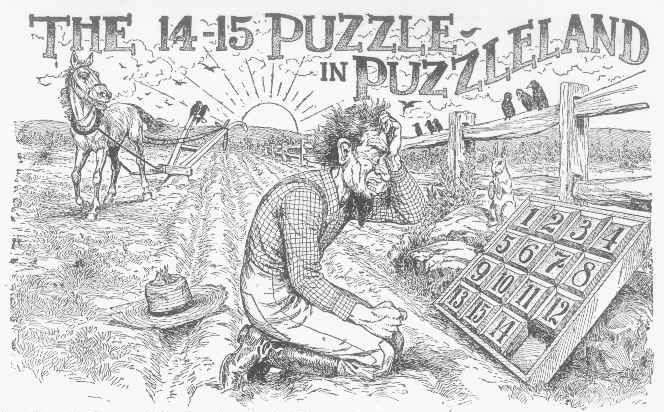
\includegraphics[width=.6\textwidth,keepaspectratio]{img/sam-loyd-puzzle-illustration.jpg}
    \captionsetup{format=hang}
    \caption[Illustration des 14-15 Puzzels von Sam Loyd]{\label{fig:puzzle-illustration}Illustration des 14-15 Puzzels von Sam Loyd (1914) \\Quelle: \cite[pp. 234-235]{loyd-cyclopedia:book}}
\end{figure}
Allerdings zeigte sich im Nachhinein, dass das Puzzel unl"osbar ist, da es eine Transformation von einer geraden zu einer ungeraden Permutation erfordert \autocite{wiki-15-puzzle:online}. Die Unl"osbarkeit des Puzzels wurde erstmals von Wm. Woolsey Johnson und William E. Story im Jahre 1879 bei einer Ver"offentlichung des American Journal of Mathematics bewiesen. \autocite{ajom-notes-15-puzzle:article}
Somit gewann keiner das Preisgeld von \$$1000$. Das 15-Puzzel wurde daraufhin auch bei einer Illustration mit dem Titel \enquote{The Great Presidential Puzzle} der US-Pr"asidentschaftswahl 1880 referenziert. Zu finden ist dies in der United States Library of Congress's Prints and Photographs division unter der Digitalen ID \textcolor{violet}{\href{https://www.loc.gov/rr/print/}{ppmsca. 15782}} \autocite{presidental-puzzle:online}.
\section{Aufgabenstellung und Abgrenzung} % (fold)
\label{cha:Aufgabenstellung}
H"atte man damals bewiesen, dass das Puzzle aus der Einleitung von Sam Loyd nicht l"osbar ist, w"are wohl vielen Menschen n"achtelange Verzweiflung erspart geblieben.\\
Nun stellt sich Frage wann eine Instanz des Puzzles l"osbar ist. Allgemein gesprochen ist eine Instanz eines 15 Puzzles dann l"osbar, falls es eine Sequenz von zul"assigen Z"ugen gibt, welche vom Startzustand zum Zielzustand f"uhren.\\
Diese Annahme gilt als Zutreffend f"ur genau die h"alfte aller m"oglichen $16! \approx 2 \cdot 10^{13}$ Puzzle Kombinationen \autocite{sliding-piece-puzzels:book,solving-15-puzzle-lvi:article}.
Das Puzzle Problem ist ein klassischer Anwendungsfall wenn es um Modellierung von Algorithmen mit Heuristiken geht. "Ublicherweise werden Algorithmen wie \textit{A*} oder \textit{IDA*} zur L"osung solcher Heurisiken genutzt \autocite{wiki-15-puzzle:online,solving-15-puzzle-lvi:article, depth-first-id:article}.
Im Rahmen dieser Arbeit geht es nun darum bei gegebener Puzzleinstanz vorherzusagen, ob diese als l"osbar oder unl"osbar gilt.
Was bei dieser Arbeit nicht betrachtet wird, sind die verschiedenen Algorithmen wie \textit{A*} oder auch \textit{IDA*}. Diese werden ausf"urhlich im zugeh"origen \textcolor{violet}{\href{https://github.com/karlstroetmann/Artificial-Intelligence/blob/master/Lecture-Notes/artificial-intelligence.pdf}{Vorlesungsskript}} \autocite{github-stroetmann:online} in den Sektionen \textit{\textbf{2.7} A* Search} und \textit{\textbf{2.10} A*-IDA* Search} erl"autert.
Lediglich werden diese genutzt um die als l"osbar identifizierten Puzzles anschlie"send auch zu l"osen.



% chapter Aufgabenstellung (end)

